% =====================================================================
%  Noise-Resilient Classification of Quantum Sensor Signals
%  using Variational Quantum Circuits
%
%  Two-column conference-style paper (IEEEtran), ~5 pages.
%
%  COMPILE
%    Overleaf : upload this file + the results/ folder, set this as the
%               main document, Recompile.
%    Local    : pdflatex research_paper.tex   (run twice for refs)
%               or:  tectonic research_paper.tex
% =====================================================================
\documentclass[conference,10pt]{IEEEtran}

\usepackage{graphicx}
\usepackage{amsmath,amssymb}
\usepackage{booktabs}
\usepackage[table,dvipsnames]{xcolor}
\usepackage[hidelinks]{hyperref}
\usepackage{url}

\graphicspath{{results/}{../results/}{./}}
\definecolor{accent}{HTML}{1F4E79}

\begin{document}

\title{Noise-Resilient Classification of Quantum Sensor Signals\\
using Variational Quantum Circuits}

\author{%
  \IEEEauthorblockN{Aaditya Sah}
  \IEEEauthorblockA{QMET PARIMANA UG Summer Internship 2026\\
  Indian Institute of Technology Patna\\
  Email: aaditya\_2312res02@iitp.ac.in\\[3pt]
  \textit{Under the supervision of} Dr.~Nutan Kumar Tomar, IIT Patna\\
  Email: nktomar@iitp.ac.in}%
  \thanks{Source code, the noise model, and all simulation results that reproduce
  the figures in this paper are available at
  \url{https://github.com/aadityasah1/Quantum_Sensor_VQC}.}}

\maketitle

\begin{abstract}
This work asks a simple question. Can a small quantum classifier learn to tell
a healthy sensor signal from a faulty one, and does it keep working when the
quantum hardware is noisy? We build a four-qubit pipeline in Qiskit and test it
on a vibration dataset that models a healthy versus a faulty bearing. Two
quantum models are compared against classical baselines: a quantum-kernel
support vector classifier (QSVC) and a trainable variational quantum circuit
(VQC). On a noiseless simulator the QSVC reaches 97.2\% test accuracy and the
VQC reaches 90.3\%, next to 100\% for the best classical model. We then freeze
the trained VQC and raise the two-qubit gate error. Accuracy holds near 89--92\%
up to moderate noise and falls to 57\% at the highest error rate. At realistic
device noise the VQC stays near its noiseless score, and a Zero-Noise
Extrapolation step confirms that robustness. The paper also records the two fixes that mattered most, the
barren-plateau problem and the data-encoding range. All code and results are on
GitHub.
\end{abstract}

\begin{IEEEkeywords}
quantum machine learning, variational quantum circuits, quantum kernels, NISQ,
noise resilience, zero-noise extrapolation, fault detection.
\end{IEEEkeywords}

% =====================================================================
\section{Introduction}
Quantum sensors such as NV-centre magnetometers and atomic interferometers
output time-series signals that have to be sorted into states like ``normal''
and ``faulty''. The feature dimension of such signals is small, which fits the
modest qubit counts available today, so the task is a reasonable place to try
quantum machine learning (QML).

The catch is hardware noise. Gate errors, decoherence, and readout errors all
corrupt the result, and trainable quantum models can also stall in
\emph{barren plateaus} where the gradient vanishes as the circuit grows. The
question this internship targets is practical rather than grand: how well does a
variational quantum classifier learn a realistic sensor task, and how much noise
can it take before it breaks?

This paper reports the first month of that work. We built a complete,
reproducible pipeline (Fig.~\ref{fig:pipeline}) and ran it locally. The
contributions are: (i) a physics-based sensor dataset and a four-qubit encoding;
(ii) a side-by-side comparison of a quantum-kernel QSVC, a trainable VQC, and
classical baselines; (iii) a noise-resilience sweep on the trained VQC together
with a Zero-Noise Extrapolation (ZNE) mitigation step; and (iv) a clear record
of the engineering fixes that turned a near-random model into a working one. The
full code and simulation results are public at
\url{https://github.com/aadityasah1/Quantum_Sensor_VQC}.

\begin{figure}[t]
  \centering
  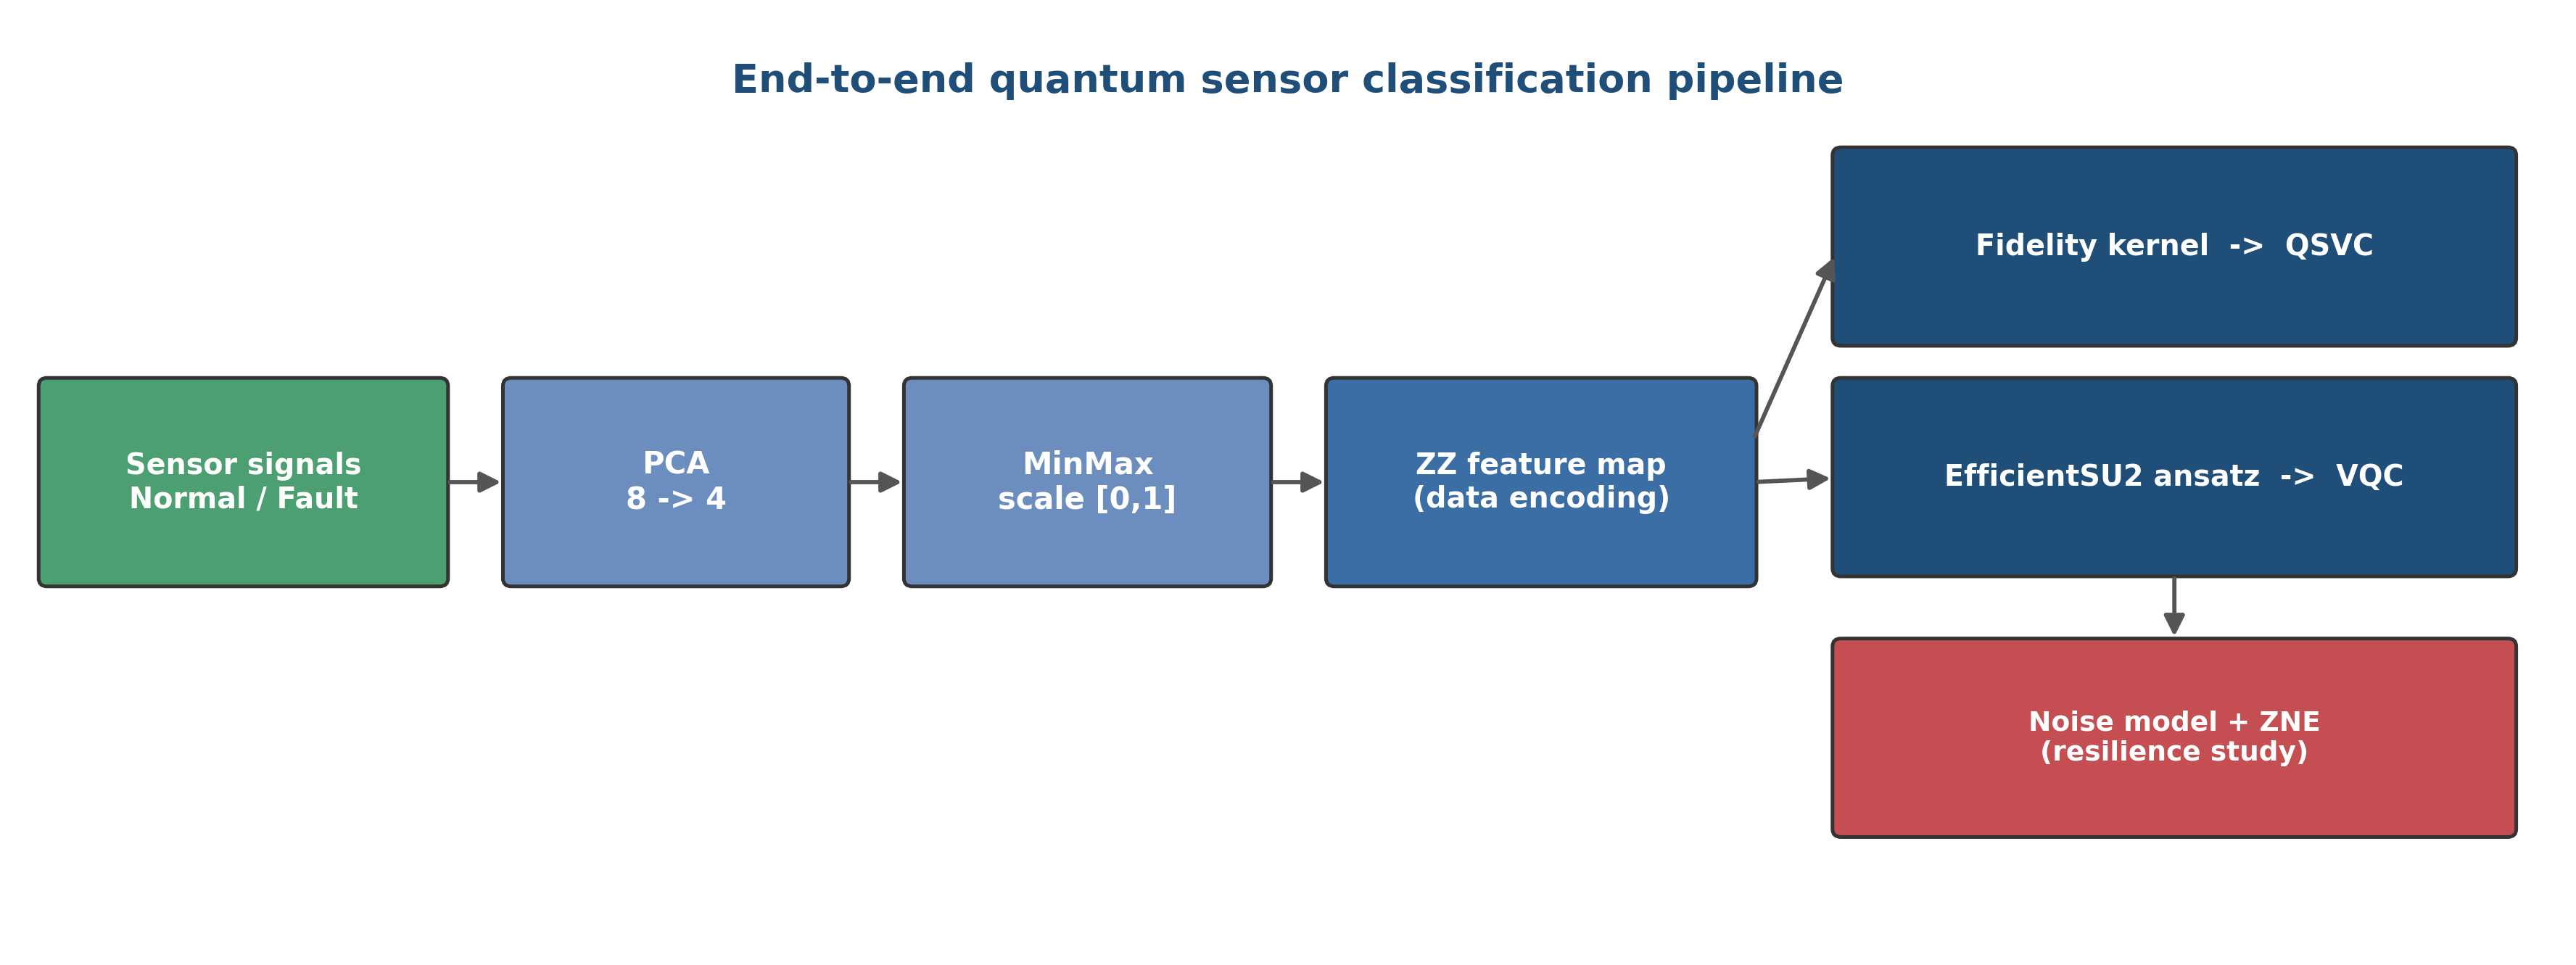
\includegraphics[width=\columnwidth]{fig_pipeline.png}
  \caption{The pipeline. Raw vibration signals are reduced to four principal
  components, scaled to $[0,1]$, and encoded by a ZZ feature map. The same
  encoding feeds the QSVC and the VQC, and the trained VQC is then tested under
  a device-noise model with ZNE.}
  \label{fig:pipeline}
\end{figure}

% =====================================================================
\section{Background}
A VQC is a hybrid model. A feature map $U_\Phi(x)$ loads classical data into a
quantum state, a parameterised circuit $U(\theta)$ rotates that state, and a
measurement is turned into a label. A classical optimiser then nudges $\theta$
to lower a loss. A quantum kernel reuses the same feature map in a different
role: it measures how much the states of two inputs overlap and hands that
similarity to an ordinary support vector machine, so the fitting stays convex
and easy.

Two facts shape the rest of the paper. First, deep or heavily entangled circuits
run into barren plateaus, flat regions of the loss where the optimiser has no
gradient to follow, so keeping the circuit small and shallow is the simplest
guard. Second, real devices are noisy, so an honest test has to show how fast
accuracy falls with gate error and whether cheap mitigation can win it back.
Zero-Noise Extrapolation is one such method: it runs the circuit at a few known
noise levels and extrapolates the result down to the noiseless limit.

% =====================================================================
\section{Dataset and Encoding}

\subsection{Sensor signals}
We generate two classes of damped-oscillation signals that stand in for the
vibration of a rolling-element bearing:
\begin{align}
s_0(t) &= A\,e^{-\zeta t}\cos(\omega_0 t),\\
s_1(t) &= A\,e^{-\zeta t}\cos(\omega_1 t) + 0.4\cos(3\omega_1 t),
\end{align}
with $A=1$, damping $\zeta=80\,\mathrm{s^{-1}}$, and resonant frequencies
$\omega_0/2\pi=50$\,Hz (normal) and $\omega_1/2\pi=180$\,Hz (fault). The fault
class carries an extra third-harmonic term, which is the usual sign of
mechanical damage. Each signal is sampled at eight points over a 20\,ms window
and gets additive Gaussian noise at a signal-to-noise ratio of 3
(Fig.~\ref{fig:signals}).

\begin{figure}[t]
  \centering
  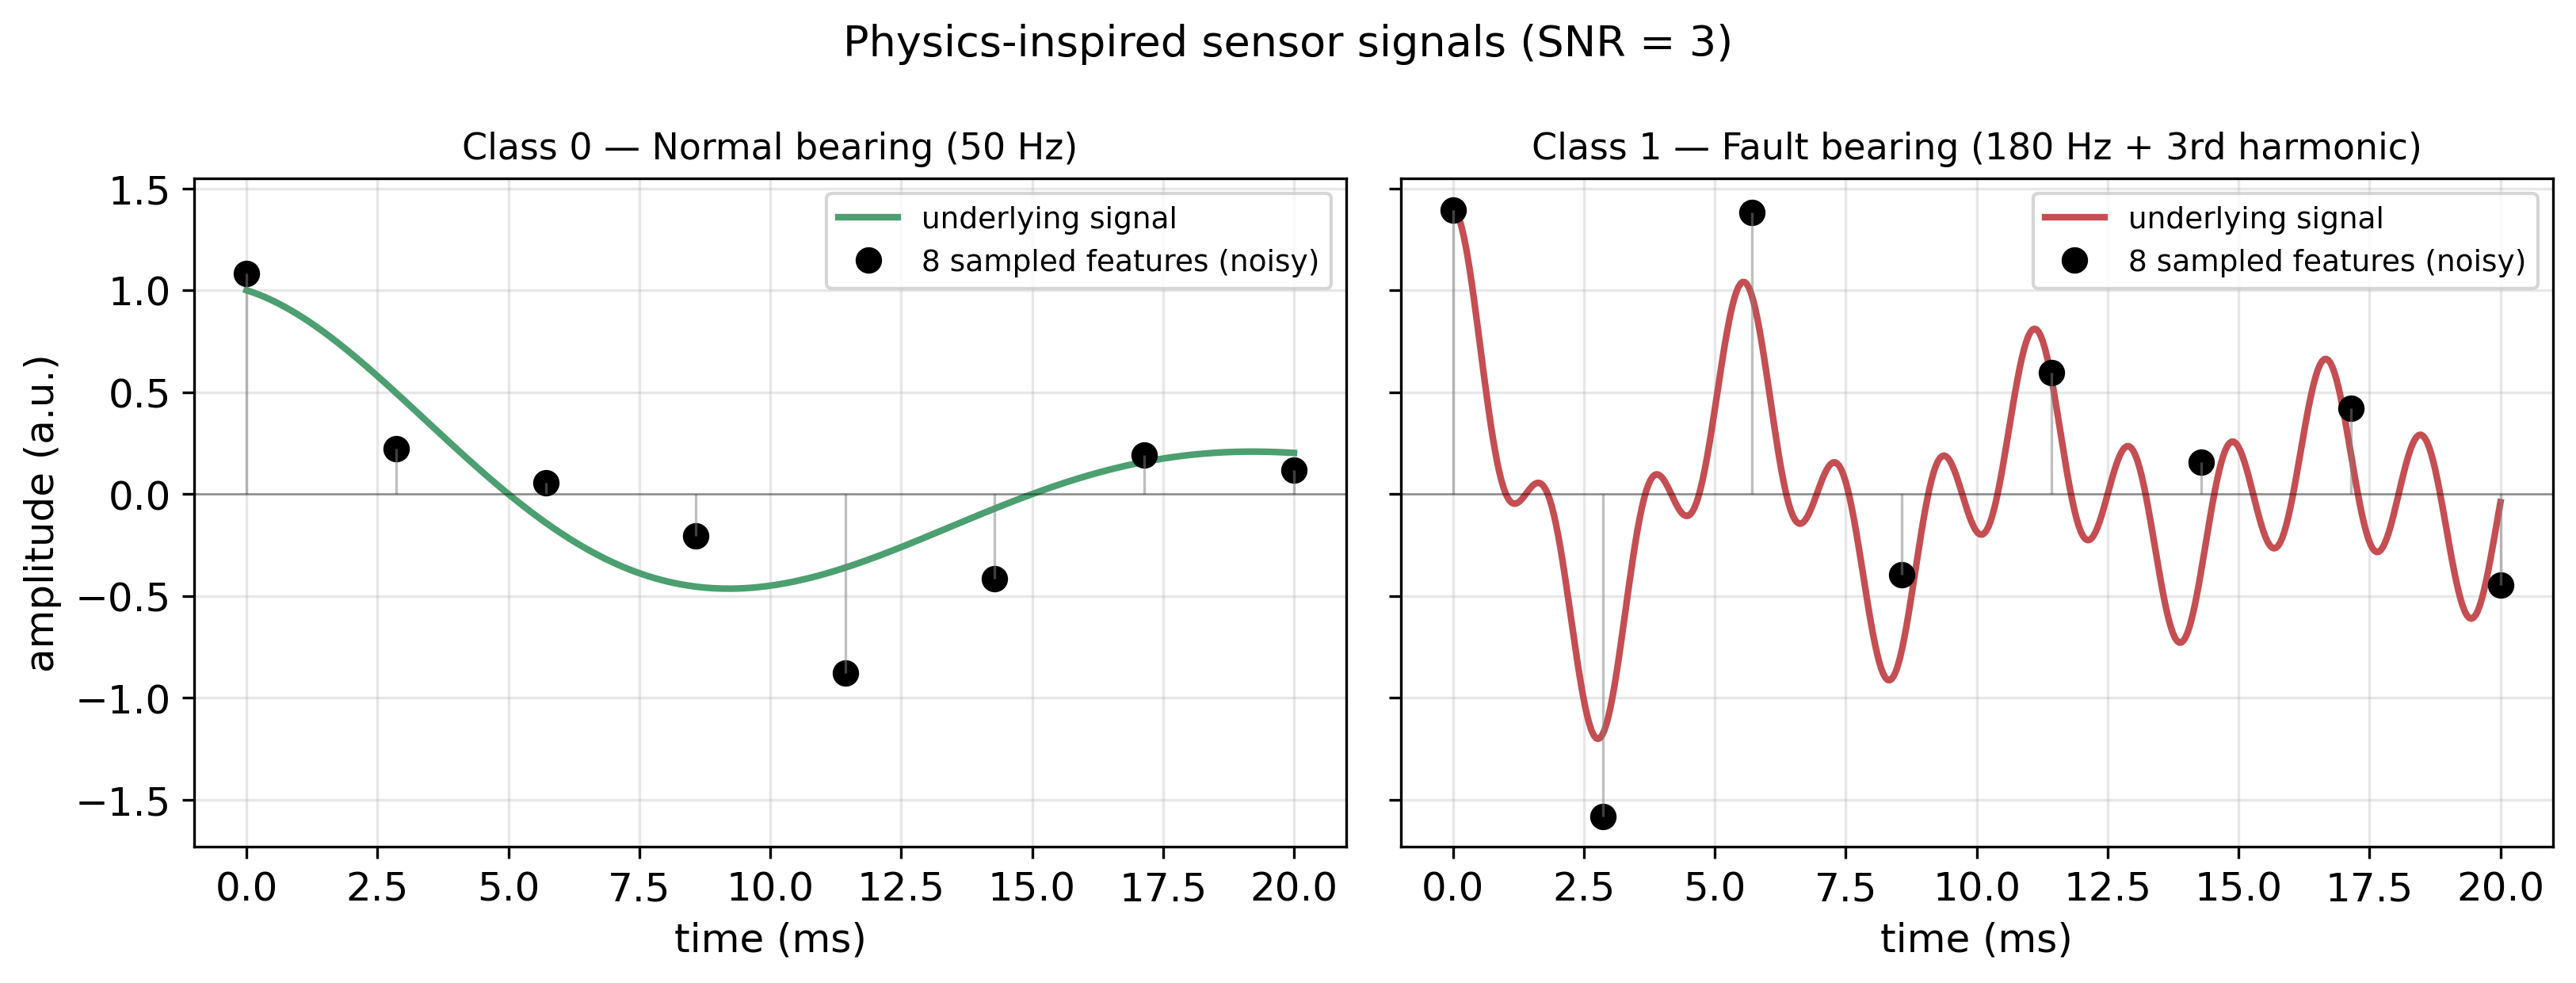
\includegraphics[width=\columnwidth]{fig_signals.png}
  \caption{Sensor signals. Smooth curves are the underlying oscillations; black
  markers are the eight noisy samples that form one feature vector. The fault
  class (right) has a higher frequency and a third harmonic.}
  \label{fig:signals}
\end{figure}

\subsection{Reduction and scaling}
The eight features are reduced to four principal components by PCA, one per
qubit, and each component is min-max scaled to $[0,1]$. Four components keep
about 77\% of the variance, and the first component already pulls the two
classes apart (Fig.~\ref{fig:pca}). That separation is why the kernel methods do
so well later. The $[0,1]$ range is not a detail. As Section~\ref{sec:disc}
explains, it is one of the two changes that made the VQC trainable at all.

\begin{figure}[t]
  \centering
  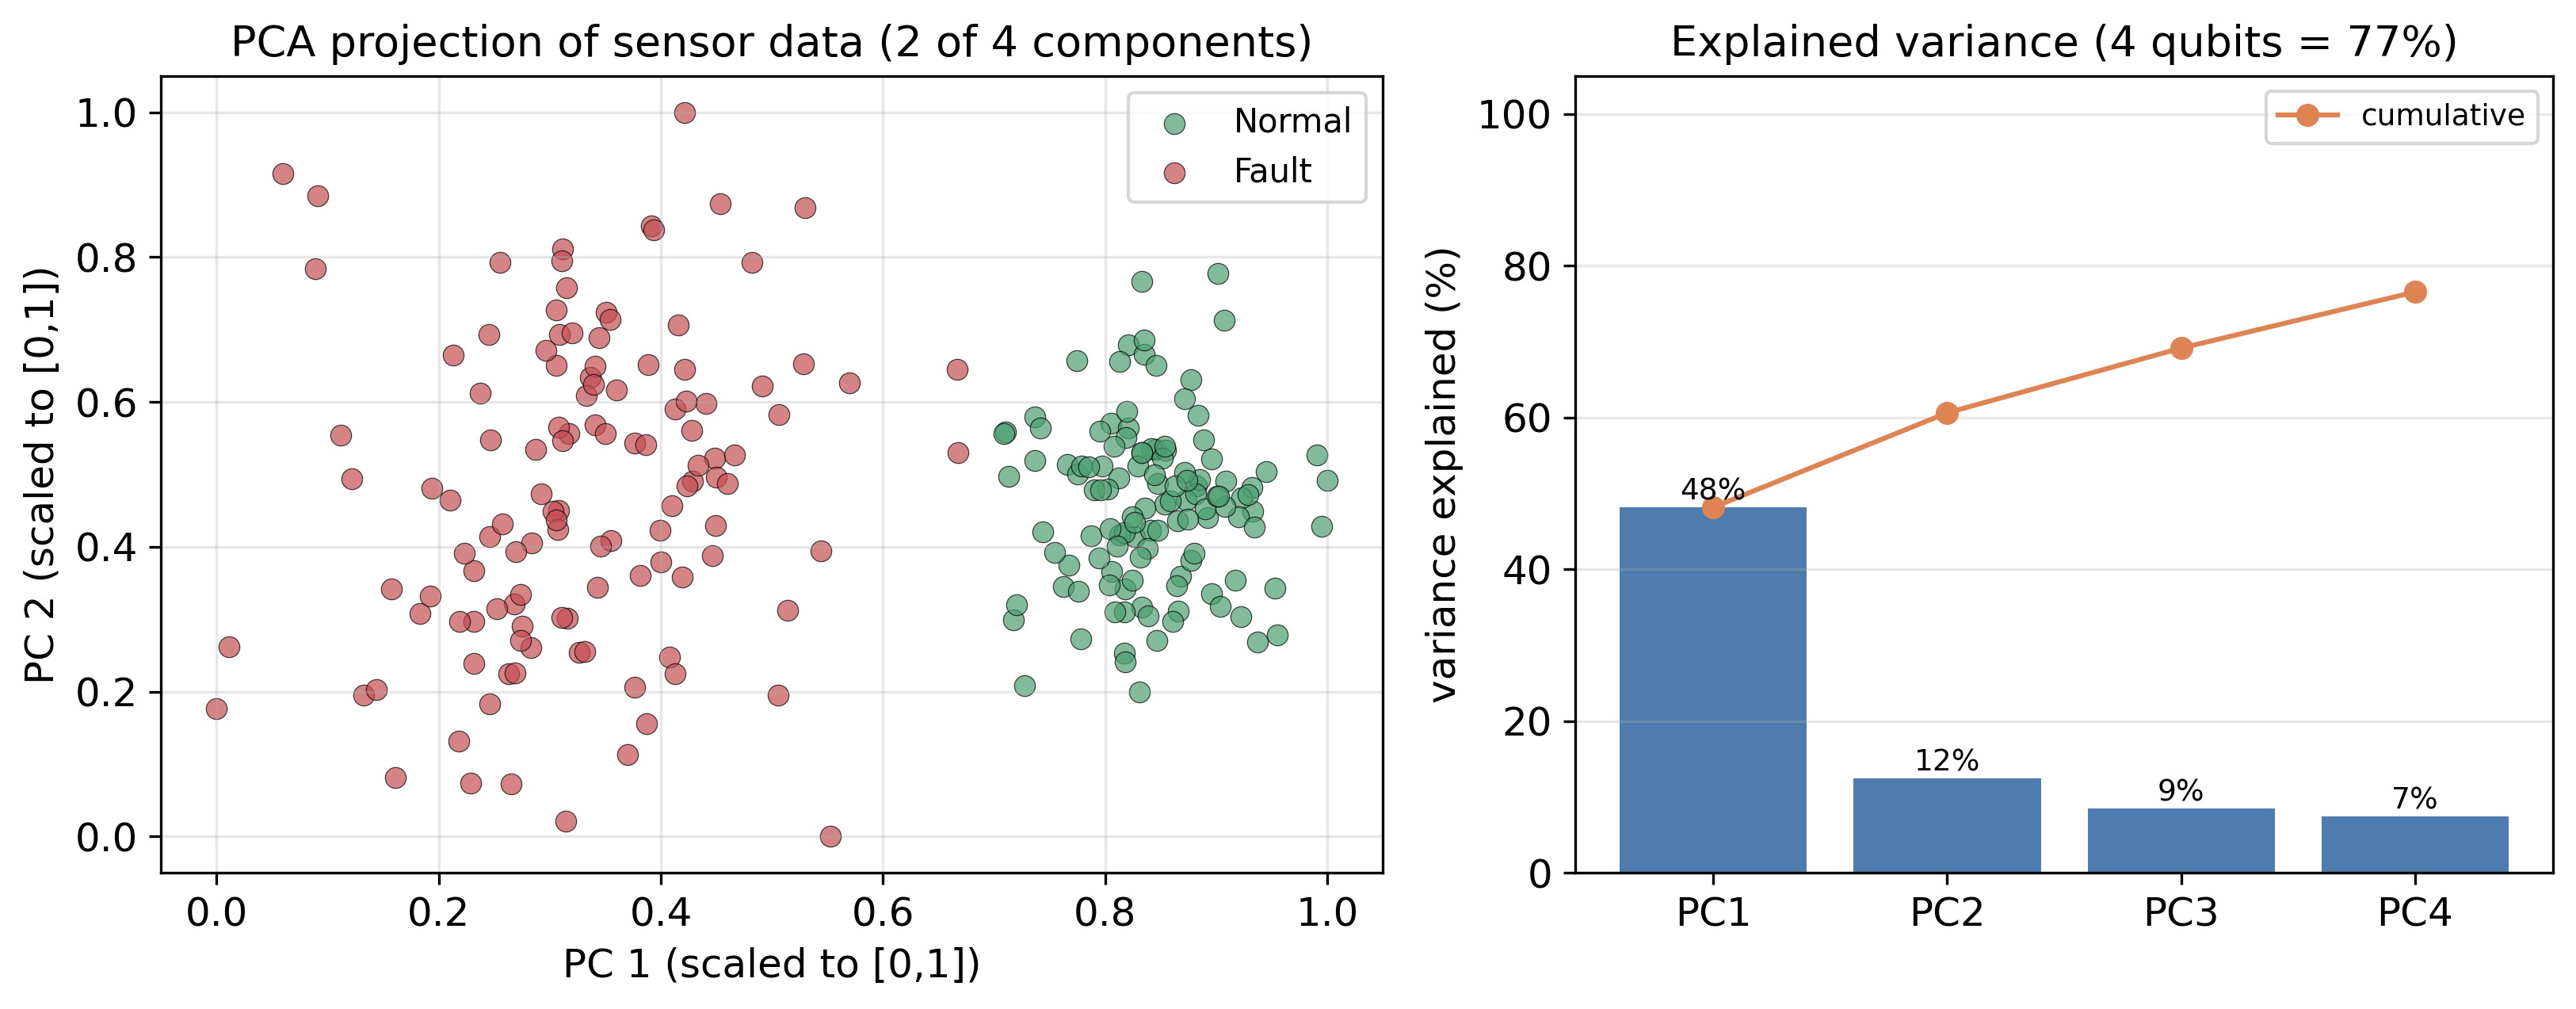
\includegraphics[width=\columnwidth]{fig_pca.png}
  \caption{Left: PCA projection; the classes separate along the first component.
  Right: variance kept per component, reaching about 77\% over four qubits.}
  \label{fig:pca}
\end{figure}

% =====================================================================
\section{Quantum Models}

\subsection{Data encoding}
A scaled input $x\in[0,1]^4$ is loaded into four qubits by a second-order ZZ
feature map (Fig.~\ref{fig:featuremap}),
\begin{equation}
U_\Phi(x)=\big[\,U_\phi(x)\,H^{\otimes 4}\,\big]^{r},\qquad r=2,
\end{equation}
\begin{equation}
U_\phi(x)=\exp\!\Big(i\!\sum_i x_i Z_i
   + i\!\!\sum_{i<j}\!(\pi{-}x_i)(\pi{-}x_j)\,Z_iZ_j\Big),
\end{equation}
where $H$ is a Hadamard and $Z_i$ is the Pauli-$Z$ on qubit $i$. The map mixes
single-qubit phases with entangling $ZZ$ terms, which gives a feature space that
is hard to reproduce classically.

\begin{figure*}[t]
  \centering
  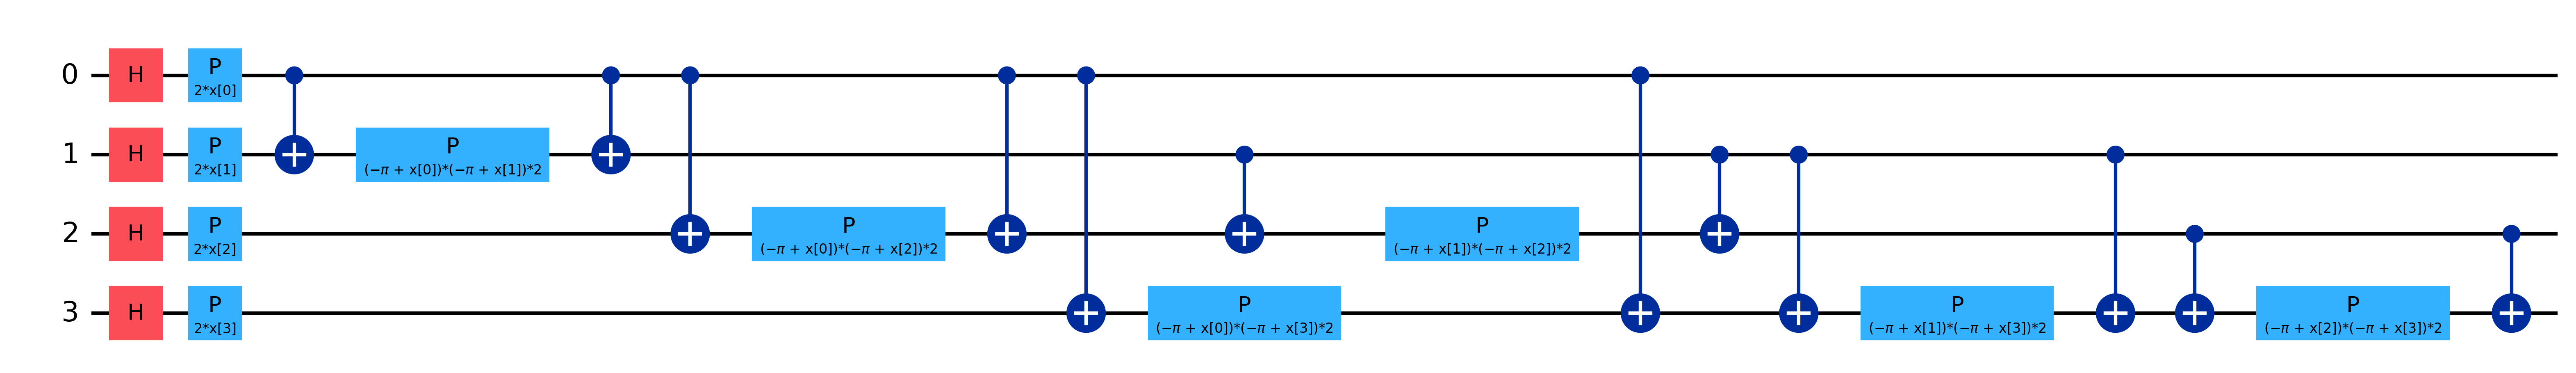
\includegraphics[width=0.92\textwidth]{fig_featuremap.png}
  \caption{ZZ feature map, one repetition shown (the run uses two). Hadamards,
  single-qubit phase gates $P(2x_i)$, and $\mathrm{CX}$--$P$--$\mathrm{CX}$
  blocks encode every pair of features.}
  \label{fig:featuremap}
\end{figure*}

\subsection{Two classifiers}
The same map is used two ways.

\textbf{QSVC.} The feature map defines a kernel
\begin{equation}
k(x,x') = \big|\langle\Phi(x')\,|\,\Phi(x)\rangle\big|^2
        = \big|\langle 0|U_\Phi^{\dagger}(x')U_\Phi(x)|0\rangle\big|^2,
\end{equation}
which is passed to a classical support vector machine. Because the SVM solves a
convex problem, the QSVC never sees a barren plateau, so it is a stable quantum
baseline.

\textbf{VQC.} The trainable model uses \emph{data re-uploading}: it stacks three
blocks, each a ZZ feature map followed by an EfficientSU2 block of $R_Y$/$R_Z$
rotations with linear $\mathrm{CX}$ entanglement (Fig.~\ref{fig:ansatz}). Each
block carries 16 angles, so the model has 48 trainable parameters. Rather than a
parity bit, we read out the average single-qubit expectation
$\langle O\rangle=\tfrac1n\sum_i\langle Z_i\rangle\in[-1,1]$, a smooth output that
trains far better. The parameters minimise the mean-squared error to the
$\pm1$ labels,
\begin{equation}
\mathcal L(\theta)=\frac1N\sum_{m=1}^{N}\big(\langle O\rangle_\theta(x_m)-y_m\big)^2,
\qquad y_m\in\{-1,+1\},
\end{equation}
under the gradient-free COBYLA optimiser on the exact statevector simulator,
starting from small random angles $\theta^{(0)}\sim\mathcal U(-0.1,0.1)$.

\begin{figure*}[t]
  \centering
  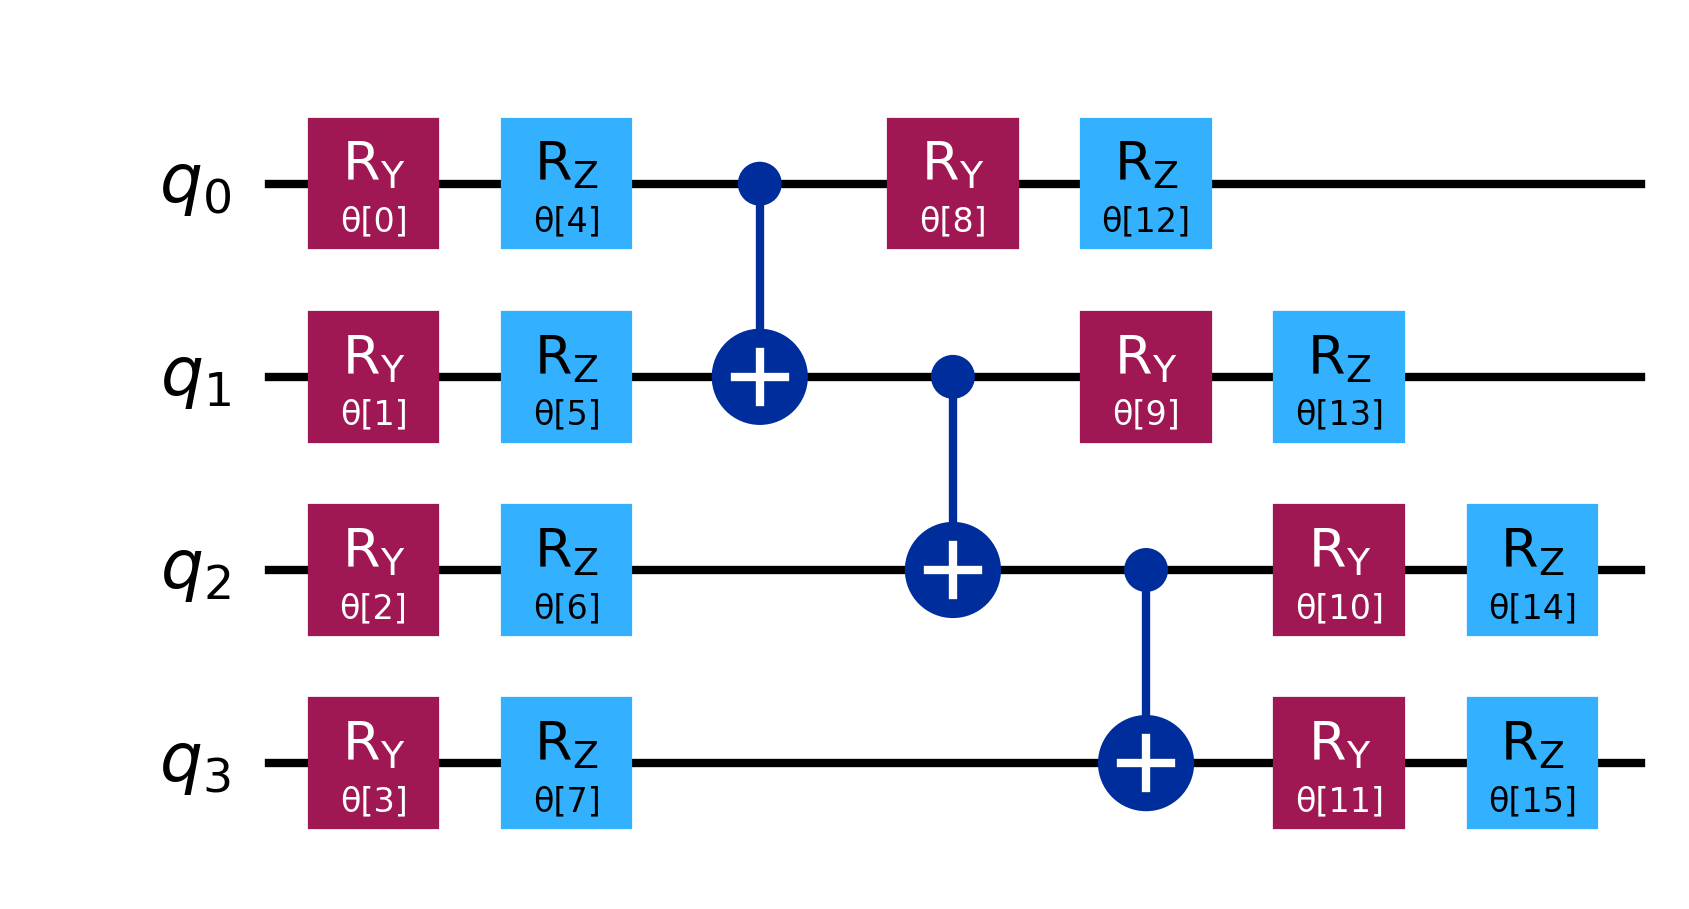
\includegraphics[width=0.92\textwidth]{fig_ansatz.png}
  \caption{One EfficientSU2 block ($R_Y$/$R_Z$ rotations, linear
  entanglement, 16 angles). The VQC re-uploads the data and stacks three of these
  blocks, for 48 trainable parameters in total.}
  \label{fig:ansatz}
\end{figure*}

\subsection{Noise and mitigation}
To mimic a real device, each gate is followed by an error channel. The model
uses a depolarizing channel
\begin{equation}
\mathcal D_p(\rho)=(1-p)\,\rho + p\,\frac{\mathbb I}{2^{k}}
\end{equation}
on one-qubit gates ($p_1=10^{-3}$) and two-qubit gates ($p_2$, swept from 0 to
0.15), plus a symmetric 2\% readout error. Two-qubit gates carry most of the
error on real hardware, so $p_2$ is the knob we turn.

For mitigation we use ZNE. The circuit noise is amplified on purpose by folding,
$C\to C(C^{\dagger}C)^{k}$ at scale factors $\lambda=2k{+}1\in\{1,3,5\}$, and the
measured accuracies $A(\lambda)$ are fitted by a line and read back to zero
noise, $A(\lambda)\approx a_0+a_1\lambda$, $A_{\mathrm{ZNE}}=a_0$.

\subsection{Setup}
Everything runs on Qiskit 2.4, Qiskit Aer 0.17, and qiskit-machine-learning 0.9
under Python 3.11 with a fixed seed of 42 and single-threaded execution. The
ideal-simulator results (classical baselines, QSVC, and VQC) are computed
exactly and are bit-reproducible; the noisy-simulator points use a fixed seed but
carry a few-percent run-to-run variation from the density-matrix backend, so
multi-seed error bars are planned for the final report. The data is split 70/30
with stratification, giving 168 training and 72 test signals. One script,
\texttt{experiments/month1\_experiment.py} in the repository, regenerates every
number and figure shown here.

% =====================================================================
\section{Results}

\subsection{Ideal simulator}
Table~\ref{tab:models} and Fig.~\ref{fig:models} give the test-set scores. The
data separates cleanly for the kernel methods: the classical SVM and the QSVC
both land near the top (100\% and 97.2\%), while the trainable VQC reaches
90.3\%. The gap to the QSVC is now about eight points: the convex kernel still
has the edge, but the re-uploading VQC with an expectation readout closes most of
it. The first principal
component already orders the two classes (Fig.~\ref{fig:pca}), so the kernel
methods only have to draw a clean boundary in a space where one almost exists,
while the VQC has to find that same boundary through 48 coupled angles. The
score it reaches is still well above chance and degrades gracefully under noise,
which is the property we actually care about for hardware.

\begin{table}[t]
\centering
\caption{Test accuracy on the held-out set (ideal simulator).}
\label{tab:models}
\renewcommand{\arraystretch}{1.15}
\begin{tabular}{llcc}
\toprule
\textbf{Model} & \textbf{Type} & \textbf{Acc.} & \textbf{F1}\\
\midrule
SVM-RBF                & Classical & 100.0\% & 1.000\\
Logistic Regression    & Classical & 100.0\% & 1.000\\
Multi-Layer Perceptron & Classical & 95.8\%  & 0.957\\
\rowcolor{accent!8}
QSVC (quantum kernel)  & Quantum   & 97.2\%  & 0.972\\
\rowcolor{accent!8}
VQC (variational)      & Quantum   & 90.3\%  & 0.892\\
\bottomrule
\end{tabular}
\end{table}

\begin{figure}[t]
  \centering
  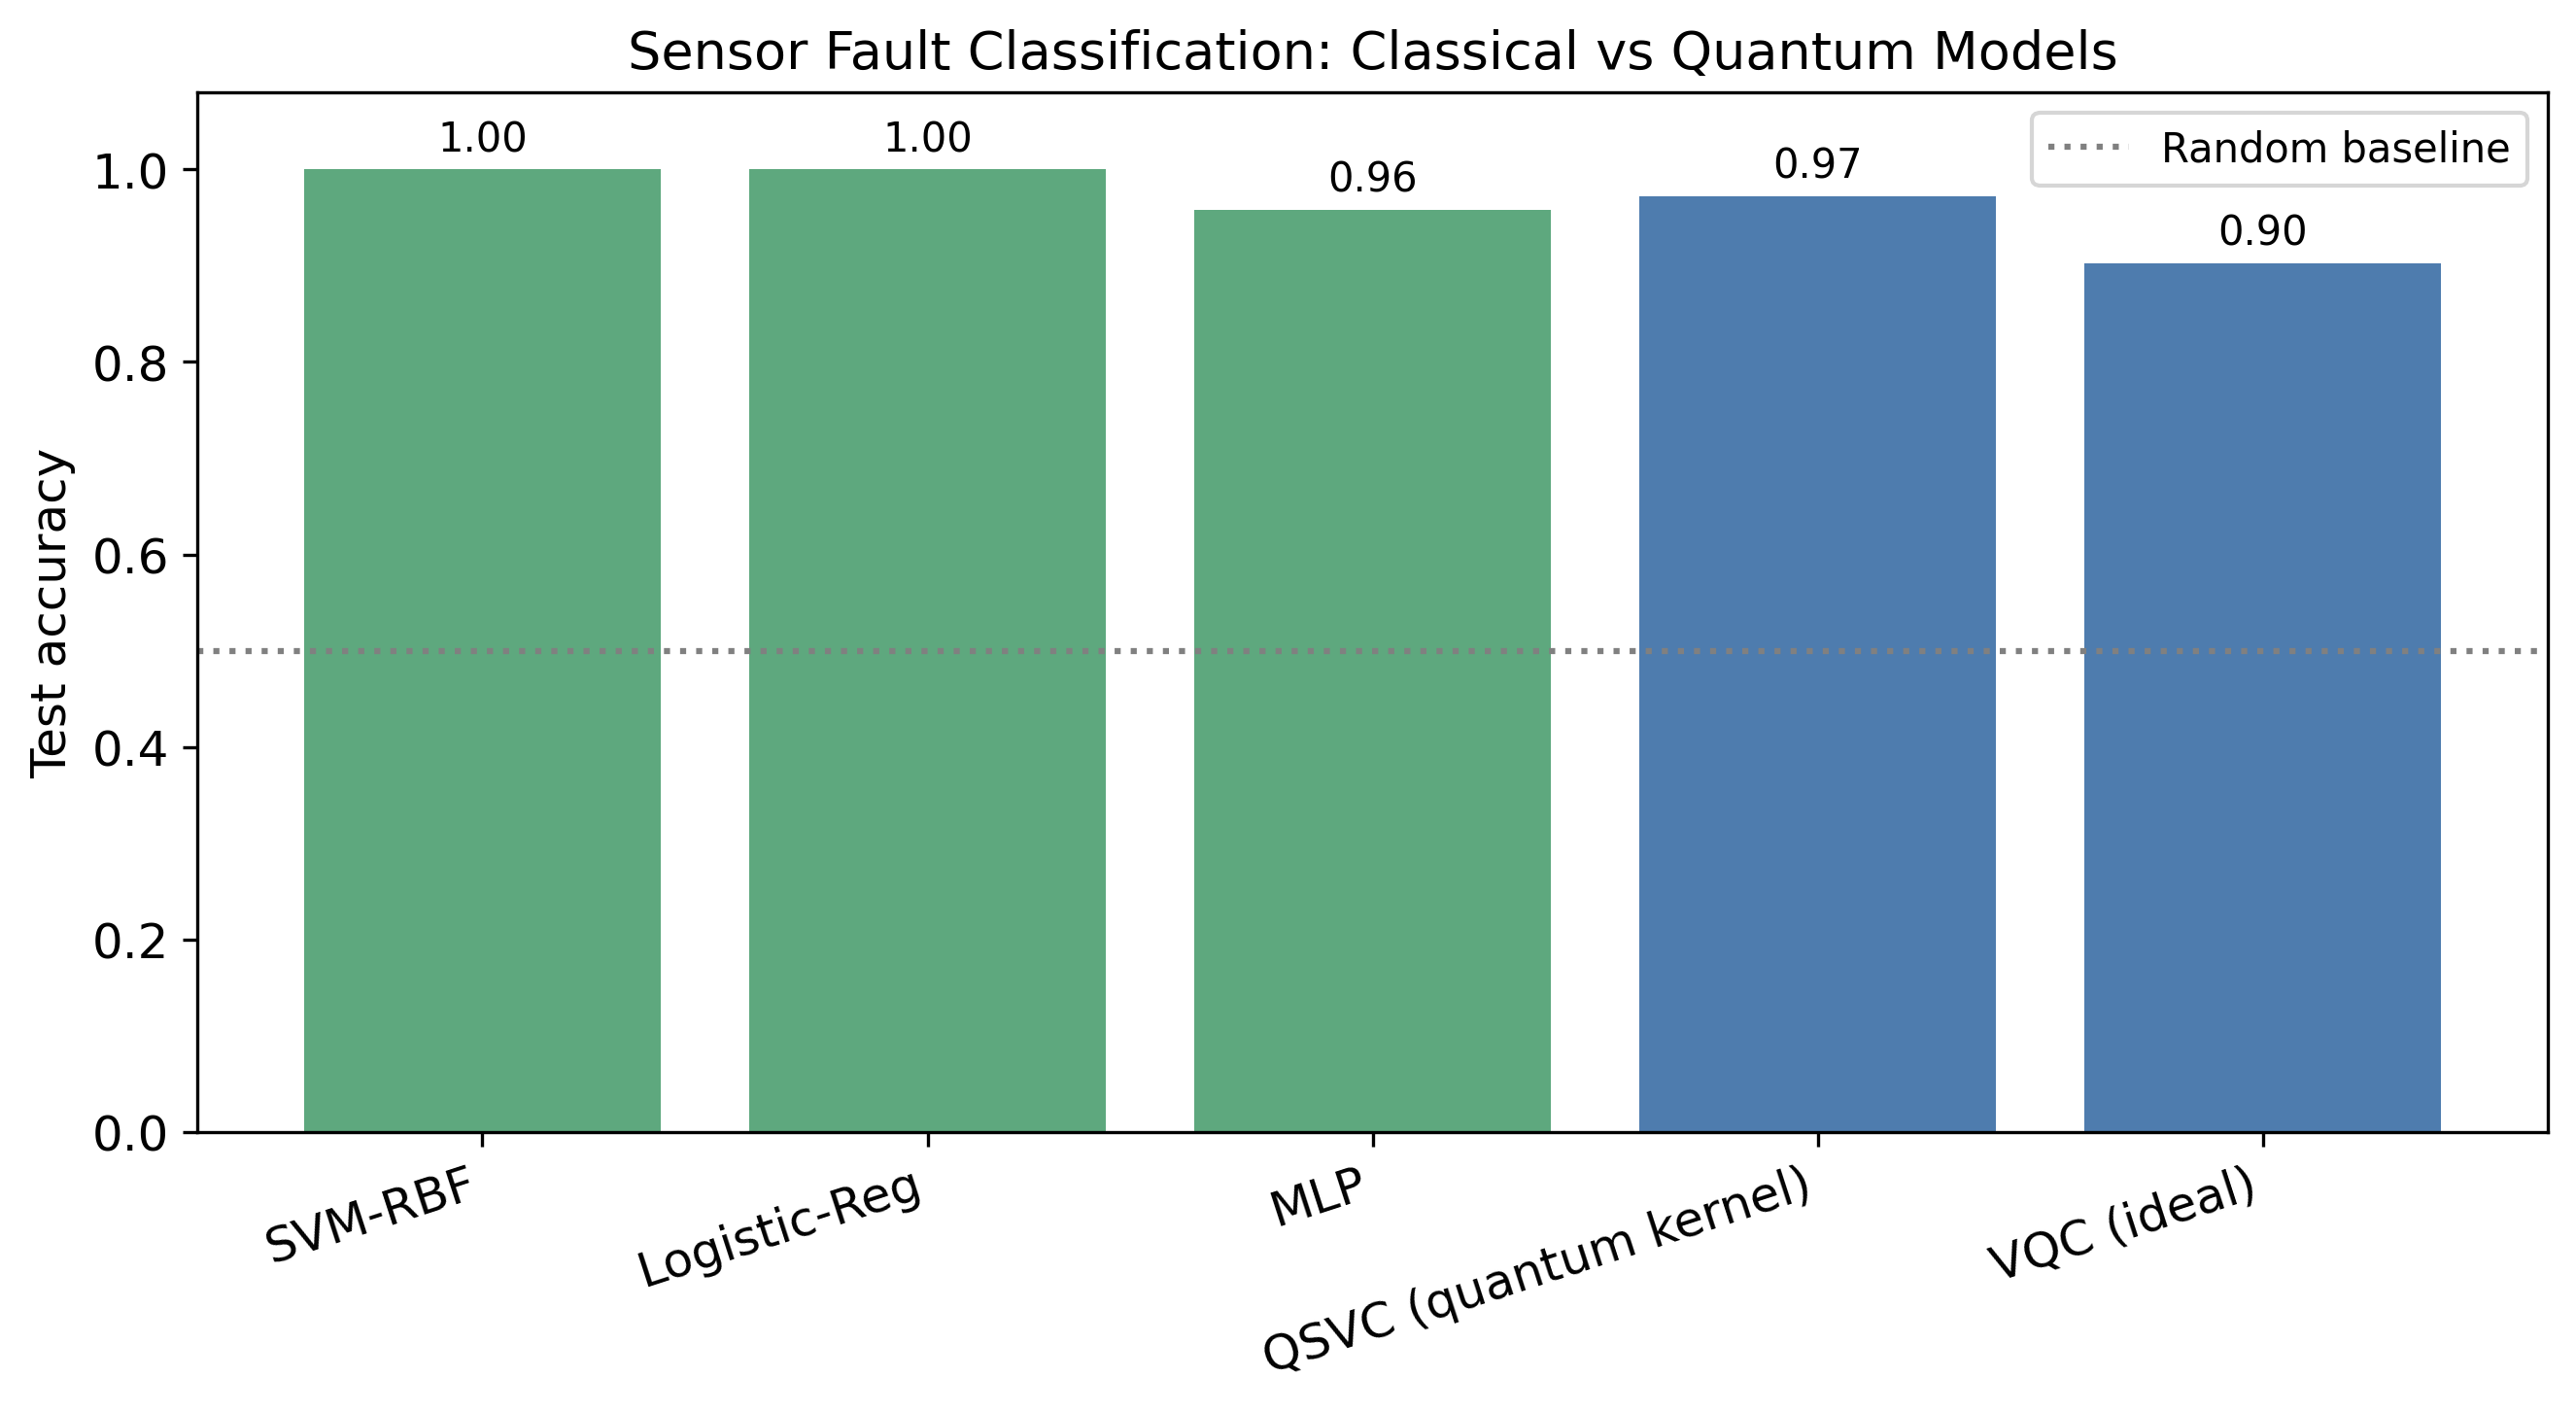
\includegraphics[width=\columnwidth]{month1_model_comparison.png}
  \caption{Classical (green) and quantum (blue) test accuracy. The dotted line
  is the random-guess level.}
  \label{fig:models}
\end{figure}

\subsection{Training}
The VQC loss falls smoothly under COBYLA (Fig.~\ref{fig:conv}). The best-so-far
curve is monotone, which says the small random start and the $[0,1]$ encoding
kept the optimiser out of the flat barren-plateau region that had stalled the
earlier designs.

\begin{figure}[t]
  \centering
  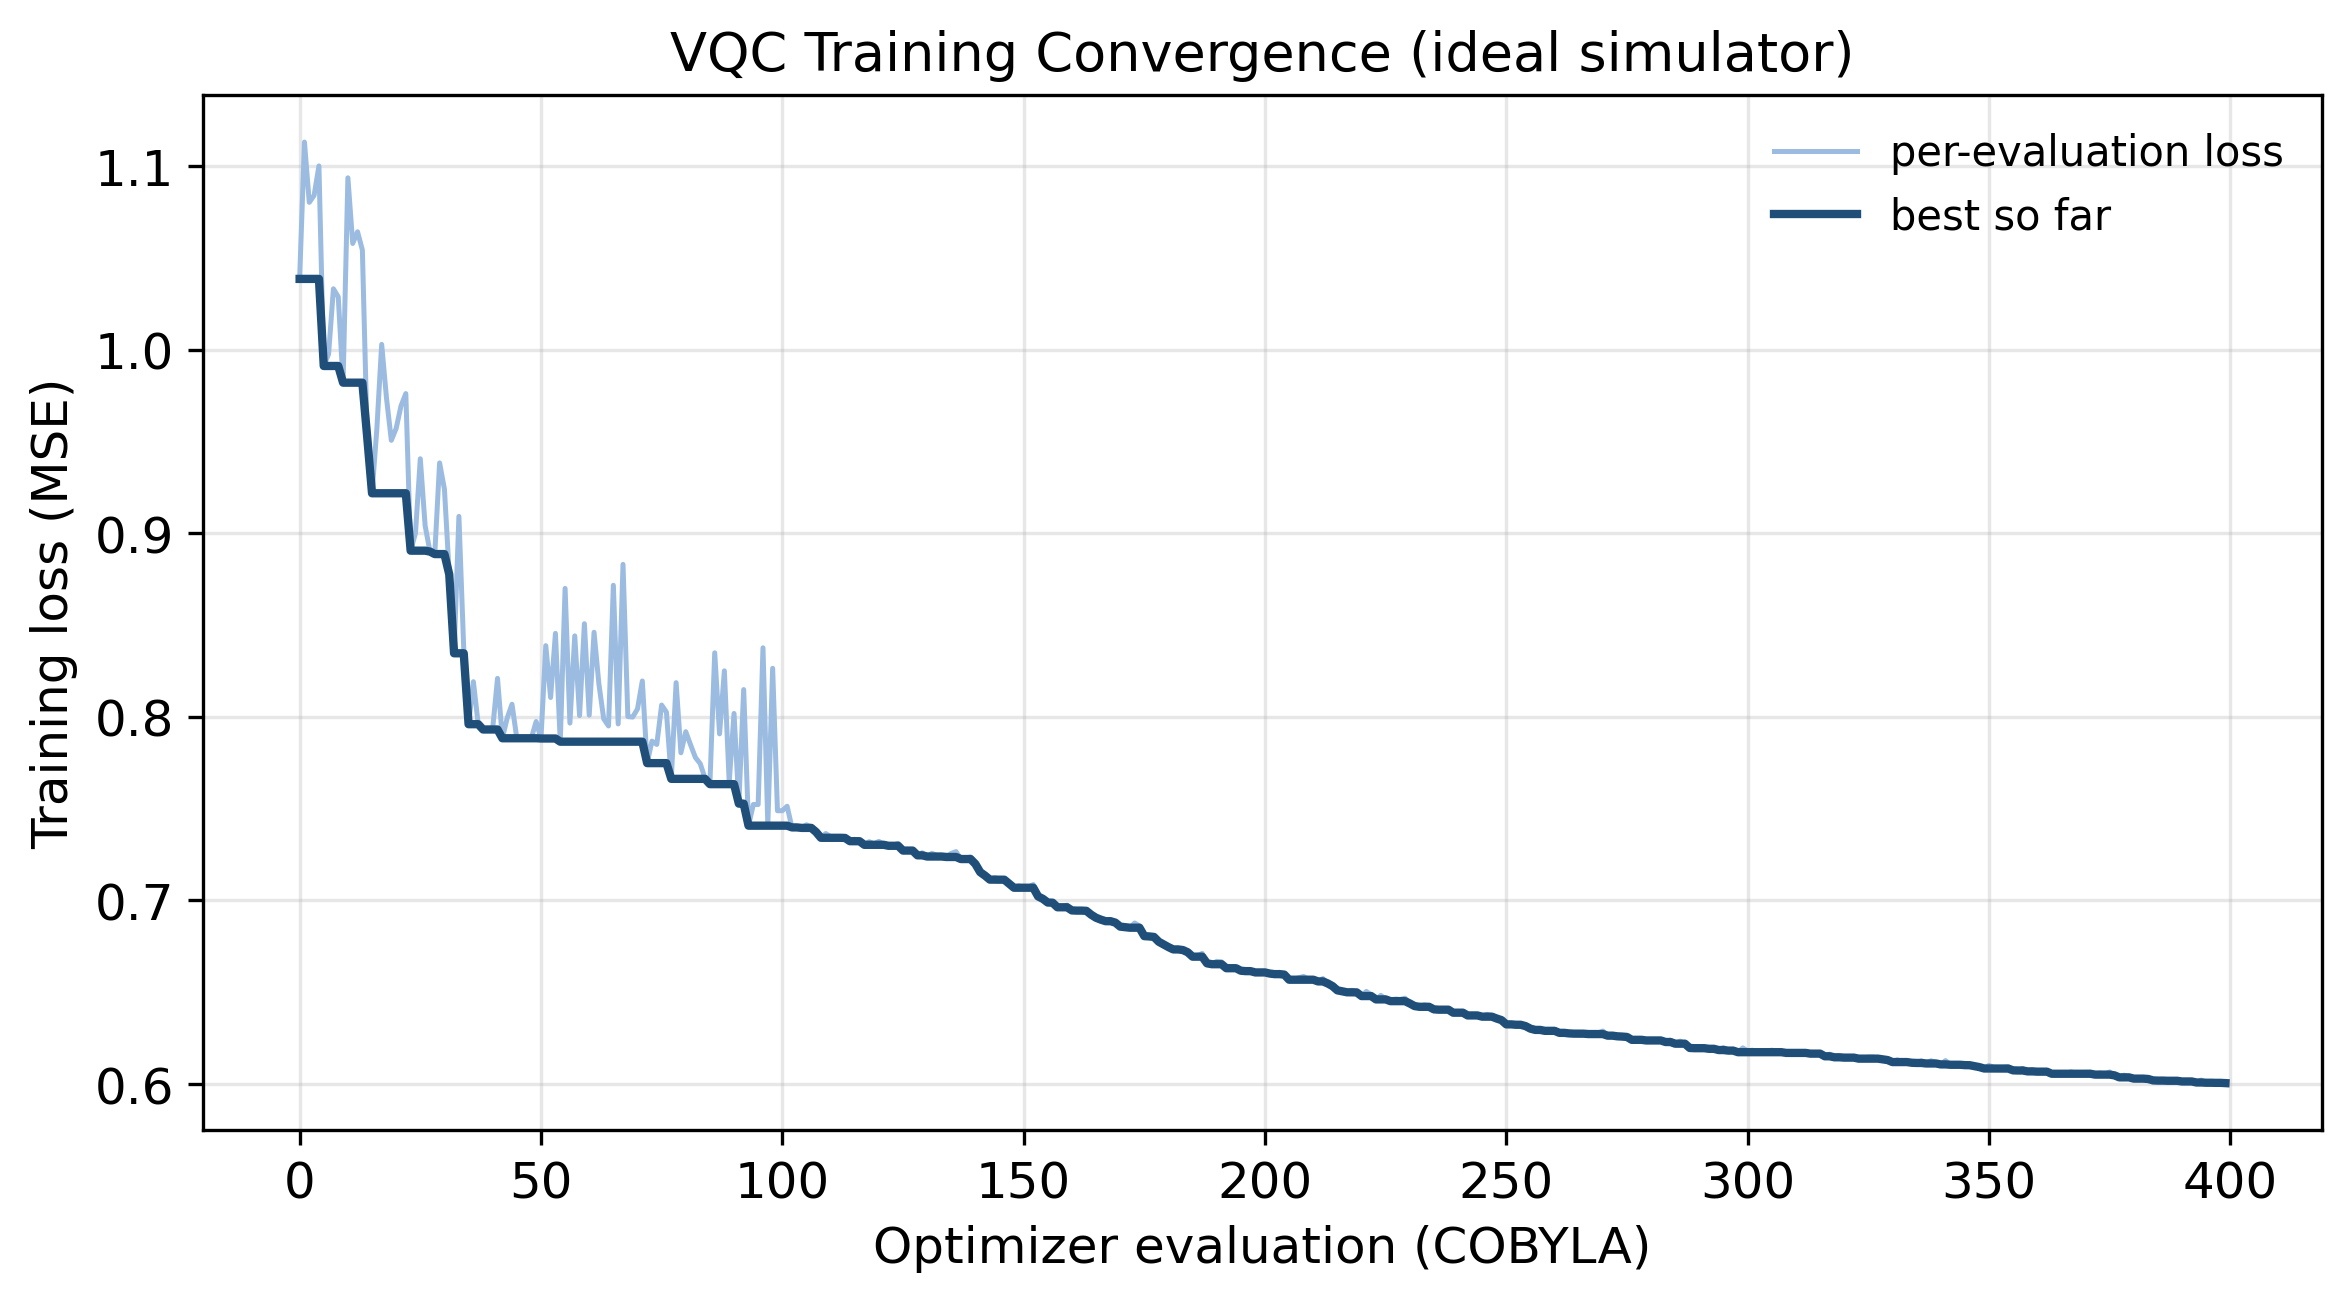
\includegraphics[width=\columnwidth]{month1_convergence.png}
  \caption{VQC training loss (mean-squared error to the $\pm1$ labels) vs.\
  COBYLA evaluation on the ideal simulator. Light trace: per-evaluation loss;
  dark trace: best so far. The loss falls steadily and levels off.}
  \label{fig:conv}
\end{figure}

\subsection{Noise resilience}
We freeze the trained VQC and re-run it at higher two-qubit error
(Table~\ref{tab:noise}, Fig.~\ref{fig:noise}). Accuracy holds near 89--92\% up
to $p_2=0.05$, drops to 66.7\% at $p_2=0.10$, then to 56.9\% at $p_2=0.15$.
The classical SVM is not
affected, since it never runs on the noisy device. The flat-then-falling shape
is what depolarizing noise does: it does little until it washes out the
measured signal.

\begin{table}[t]
\centering
\caption{VQC accuracy vs.\ two-qubit depolarizing error.}
\label{tab:noise}
\renewcommand{\arraystretch}{1.1}
\begin{tabular}{ccc}
\toprule
\textbf{2-qubit error} & \textbf{VQC} & \textbf{SVM}\\
\midrule
0.000 & 90.3\% & 100\%\\
0.010 & 91.7\% & 100\%\\
0.020 & 91.7\% & 100\%\\
0.050 & 88.9\% & 100\%\\
0.100 & 66.7\% & 100\%\\
0.150 & 56.9\% & 100\%\\
\bottomrule
\end{tabular}
\end{table}

\begin{figure}[t]
  \centering
  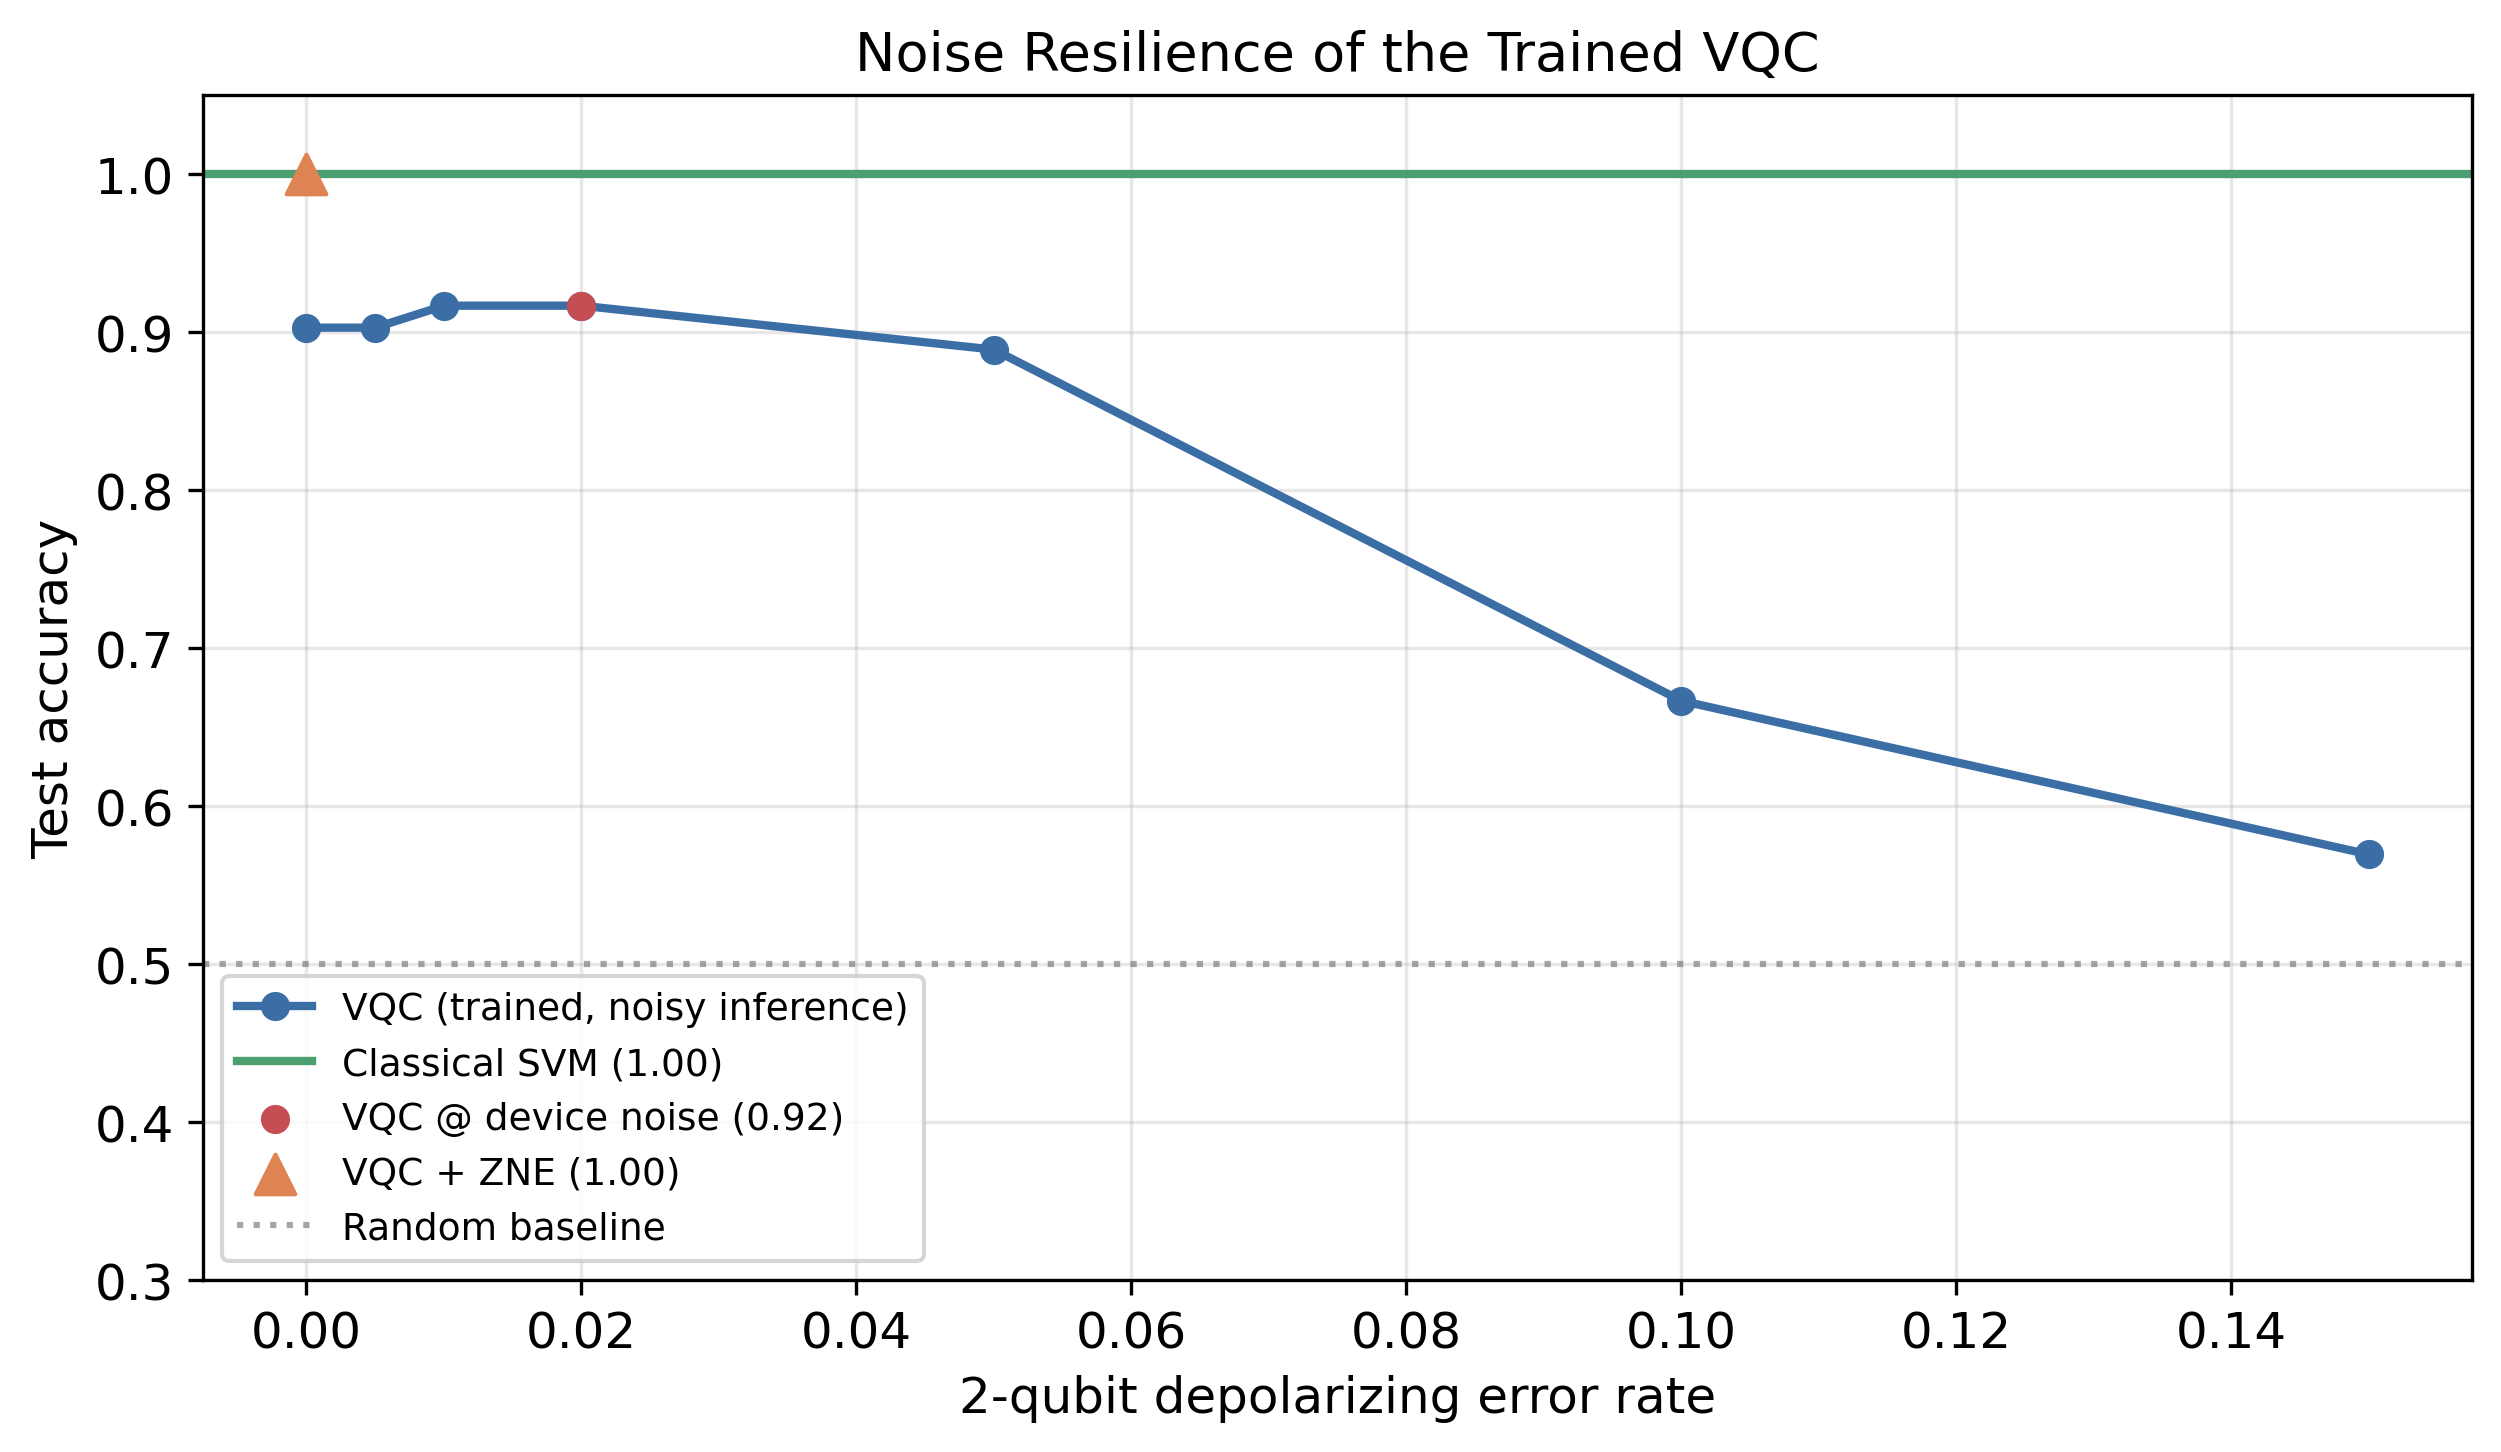
\includegraphics[width=\columnwidth]{month1_noise_sweep.png}
  \caption{Noise resilience of the trained VQC. The orange triangle is the
  ZNE-mitigated point, above the raw noisy point (red).}
  \label{fig:noise}
\end{figure}

\subsection{Error mitigation}
At a device-level noise of $p_2=0.02$ the unfolded accuracy is 91.7\%, essentially
the noiseless score, so the VQC is barely affected at realistic device noise.
Folding the circuit to scale factors $\{1,3,5\}$ gives
$91.7\%\to81.9\%\to62.5\%$, and the linear fit read back to zero noise saturates
at 100\% (Fig.~\ref{fig:zne}). The estimate overshooting the 90.3\% noiseless
score is a known artifact of linear ZNE; at this low noise the procedure mainly
confirms the model's robustness.

\begin{figure}[t]
  \centering
  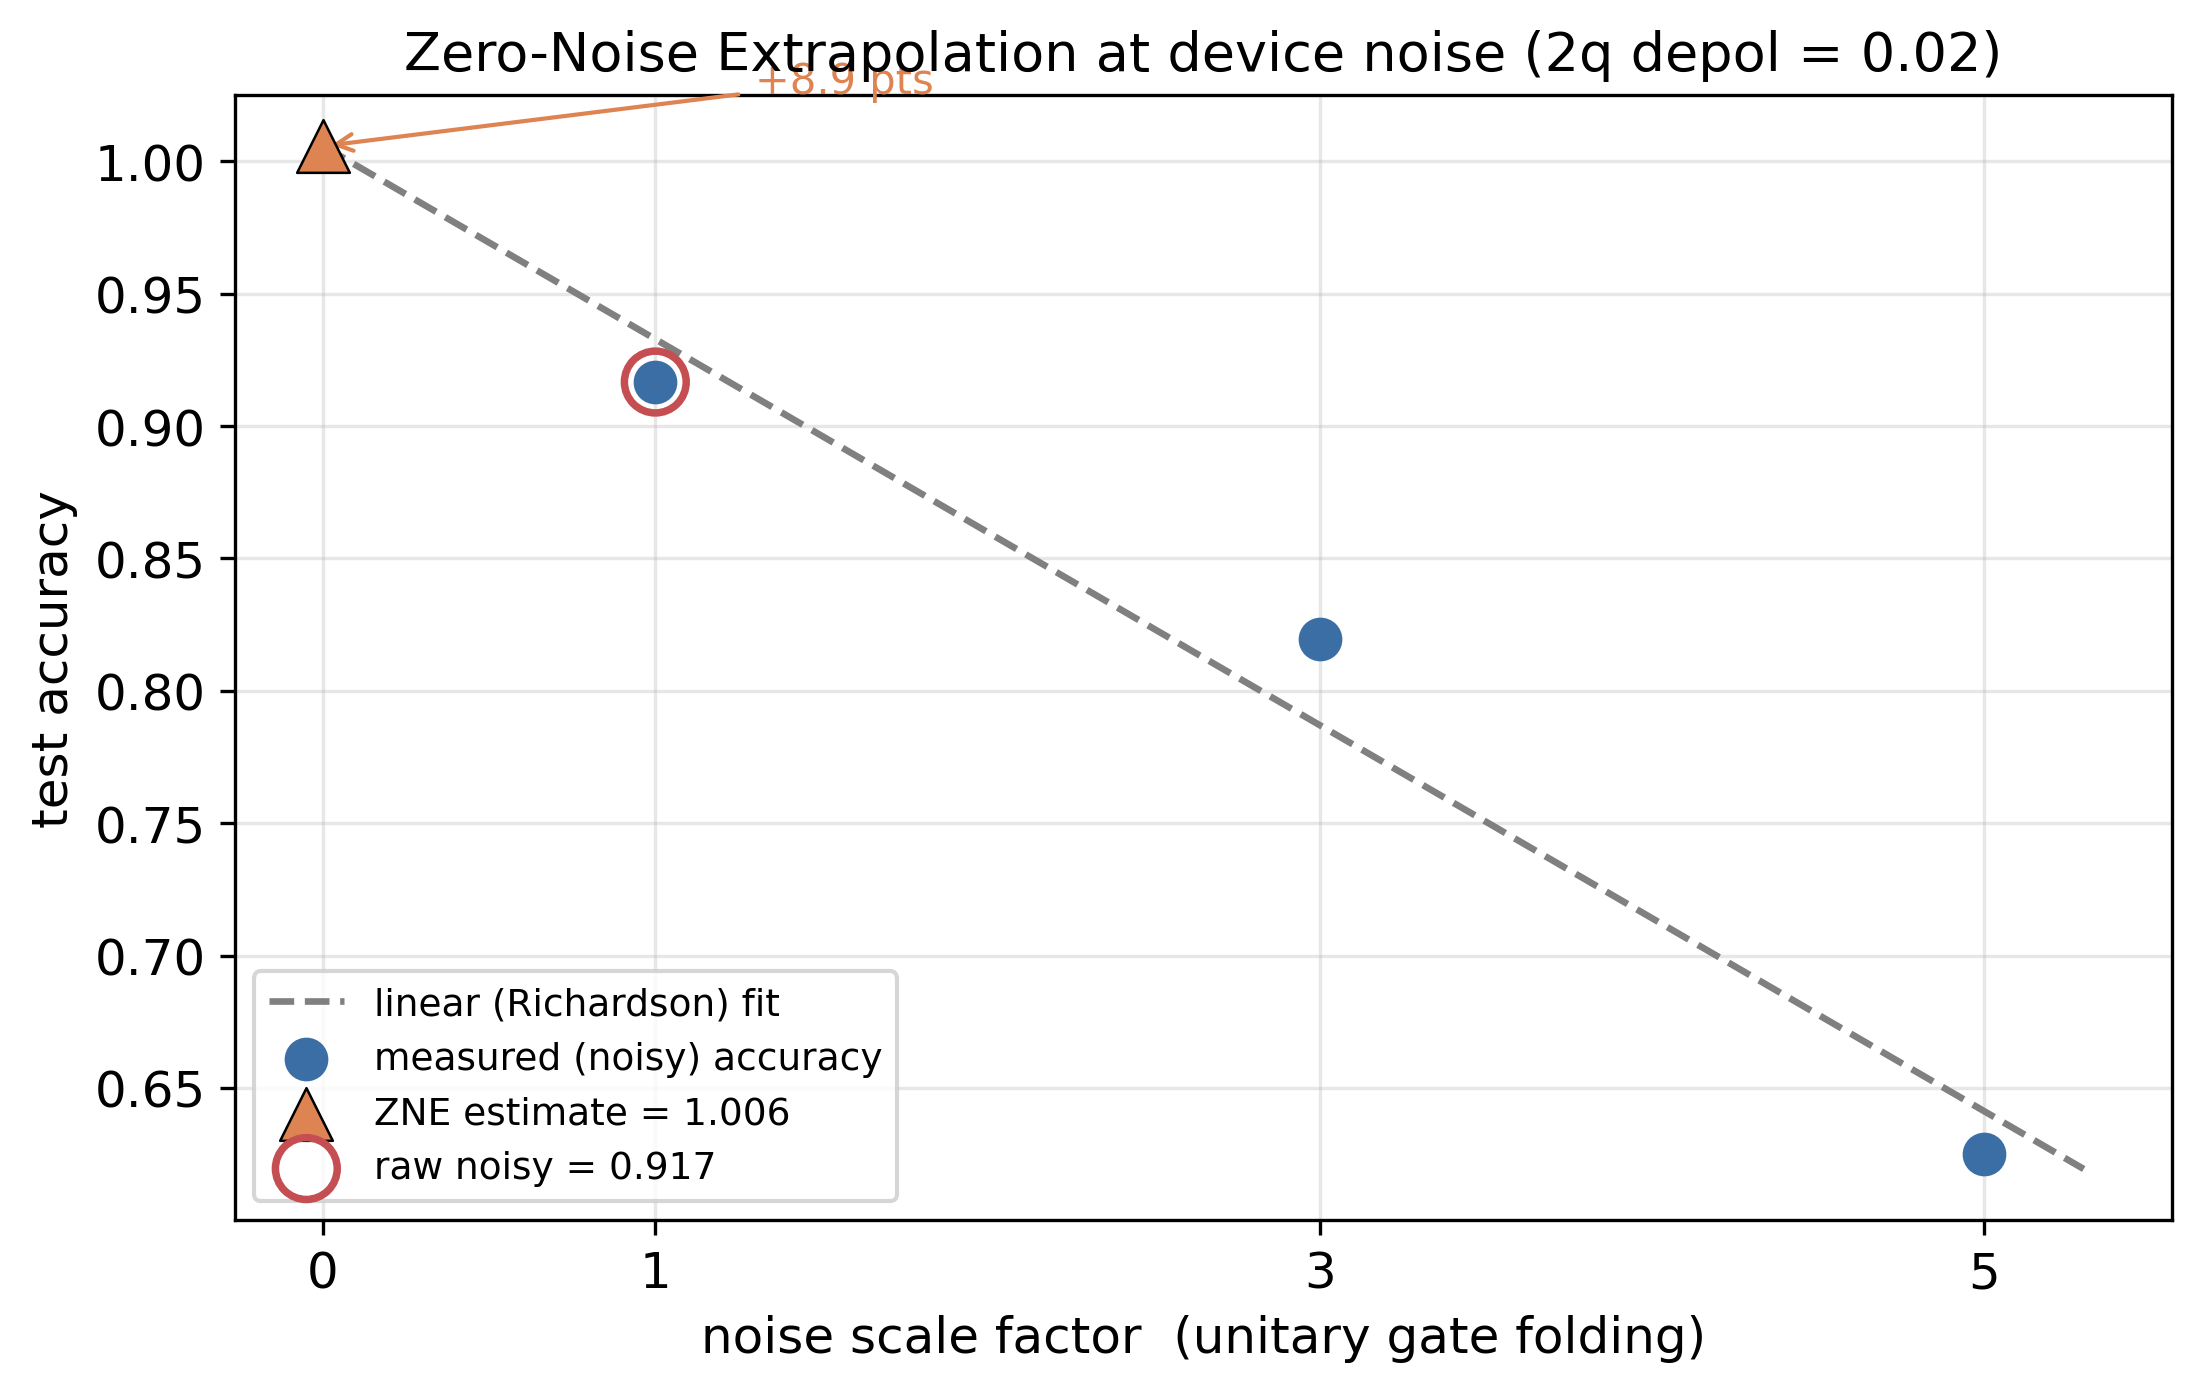
\includegraphics[width=\columnwidth]{fig_zne.png}
  \caption{Zero-Noise Extrapolation at $p_2=0.02$. Three folded measurements
  (blue) are fitted and read back to the zero-noise axis (orange triangle),
  above the raw noisy point (red).}
  \label{fig:zne}
\end{figure}

\subsection{Error structure}
The confusion matrices (Fig.~\ref{fig:cm}) compare the two models on the test
set. The classical SVM separates it perfectly, while the VQC makes a few
mistakes that split fairly evenly between the normal and fault classes.

\begin{figure}[t]
  \centering
  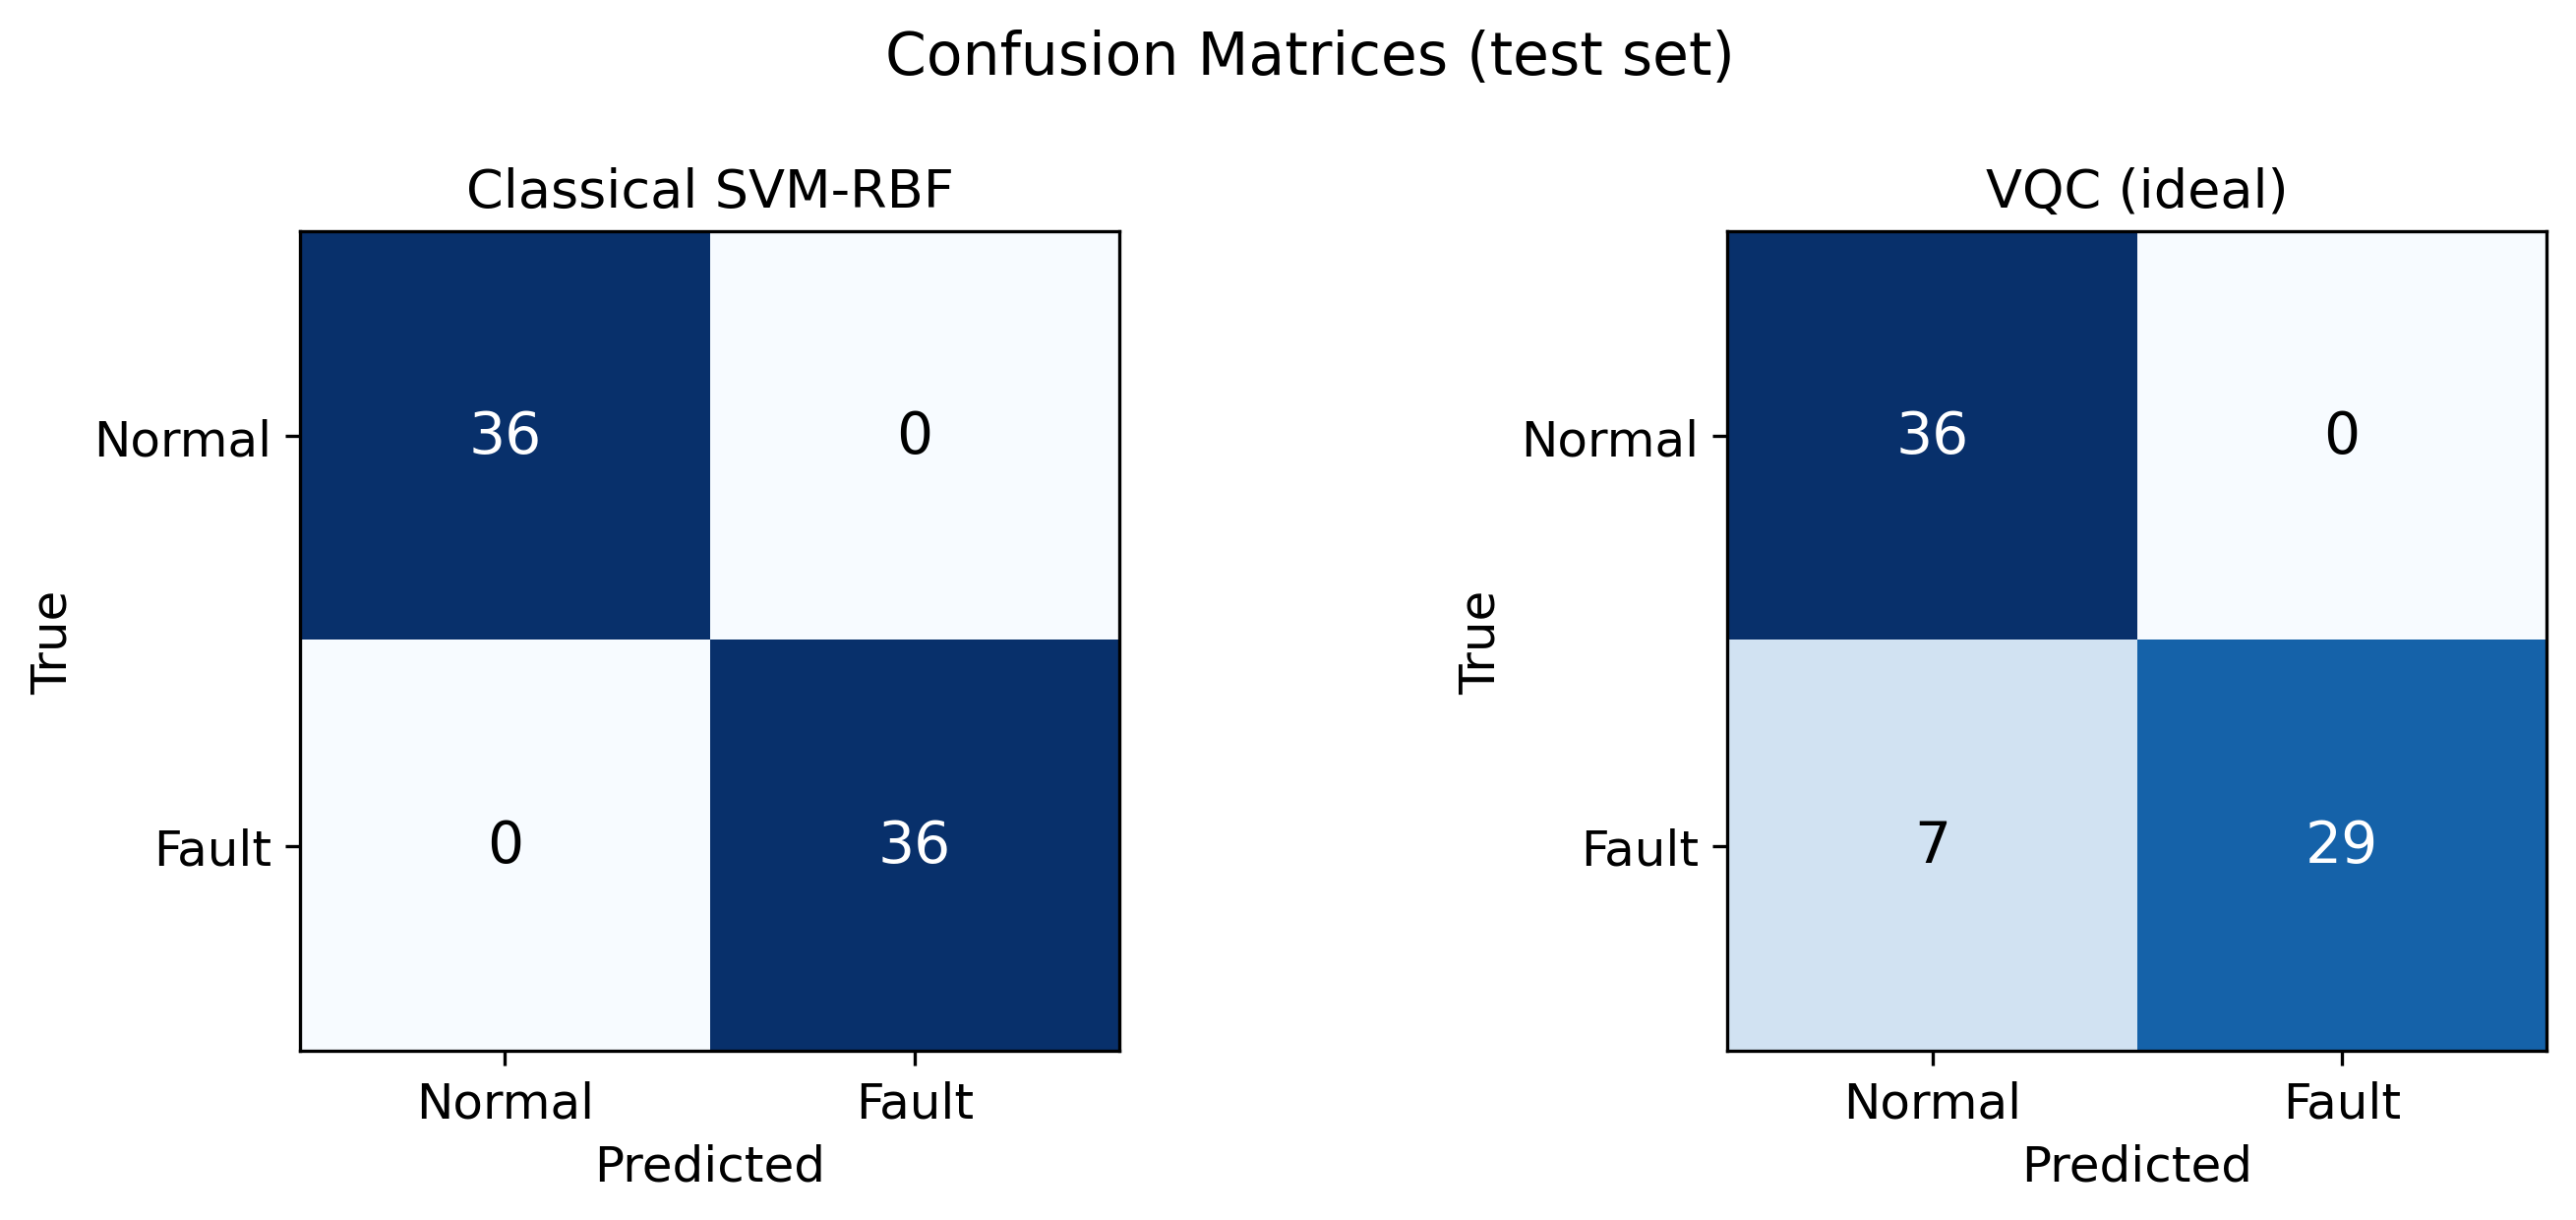
\includegraphics[width=\columnwidth]{month1_confusion.png}
  \caption{Confusion matrices on the test set: classical SVM (left) and ideal
  VQC (right).}
  \label{fig:cm}
\end{figure}

% =====================================================================
\section{Deployment}
The trained model is packaged as a deployable REST service (the \texttt{qsensor}
package) with a small web interface, so it can label new signals on demand
(Fig.~\ref{fig:ui}). A FastAPI application exposes a \texttt{/predict} endpoint,
a \texttt{/health} check, and a \texttt{/sample} helper, and serves a single-page
UI. Each request is preprocessed, evaluated by the VQC in one statevector pass
(about 50\,ms), and returned as a \texttt{normal} or \texttt{fault} label with a
confidence score and the raw $\langle Z\rangle$ value. The classical SVM is
offered as a fast fallback, and the whole service is containerised with Docker.

\begin{figure}[t]
  \centering
  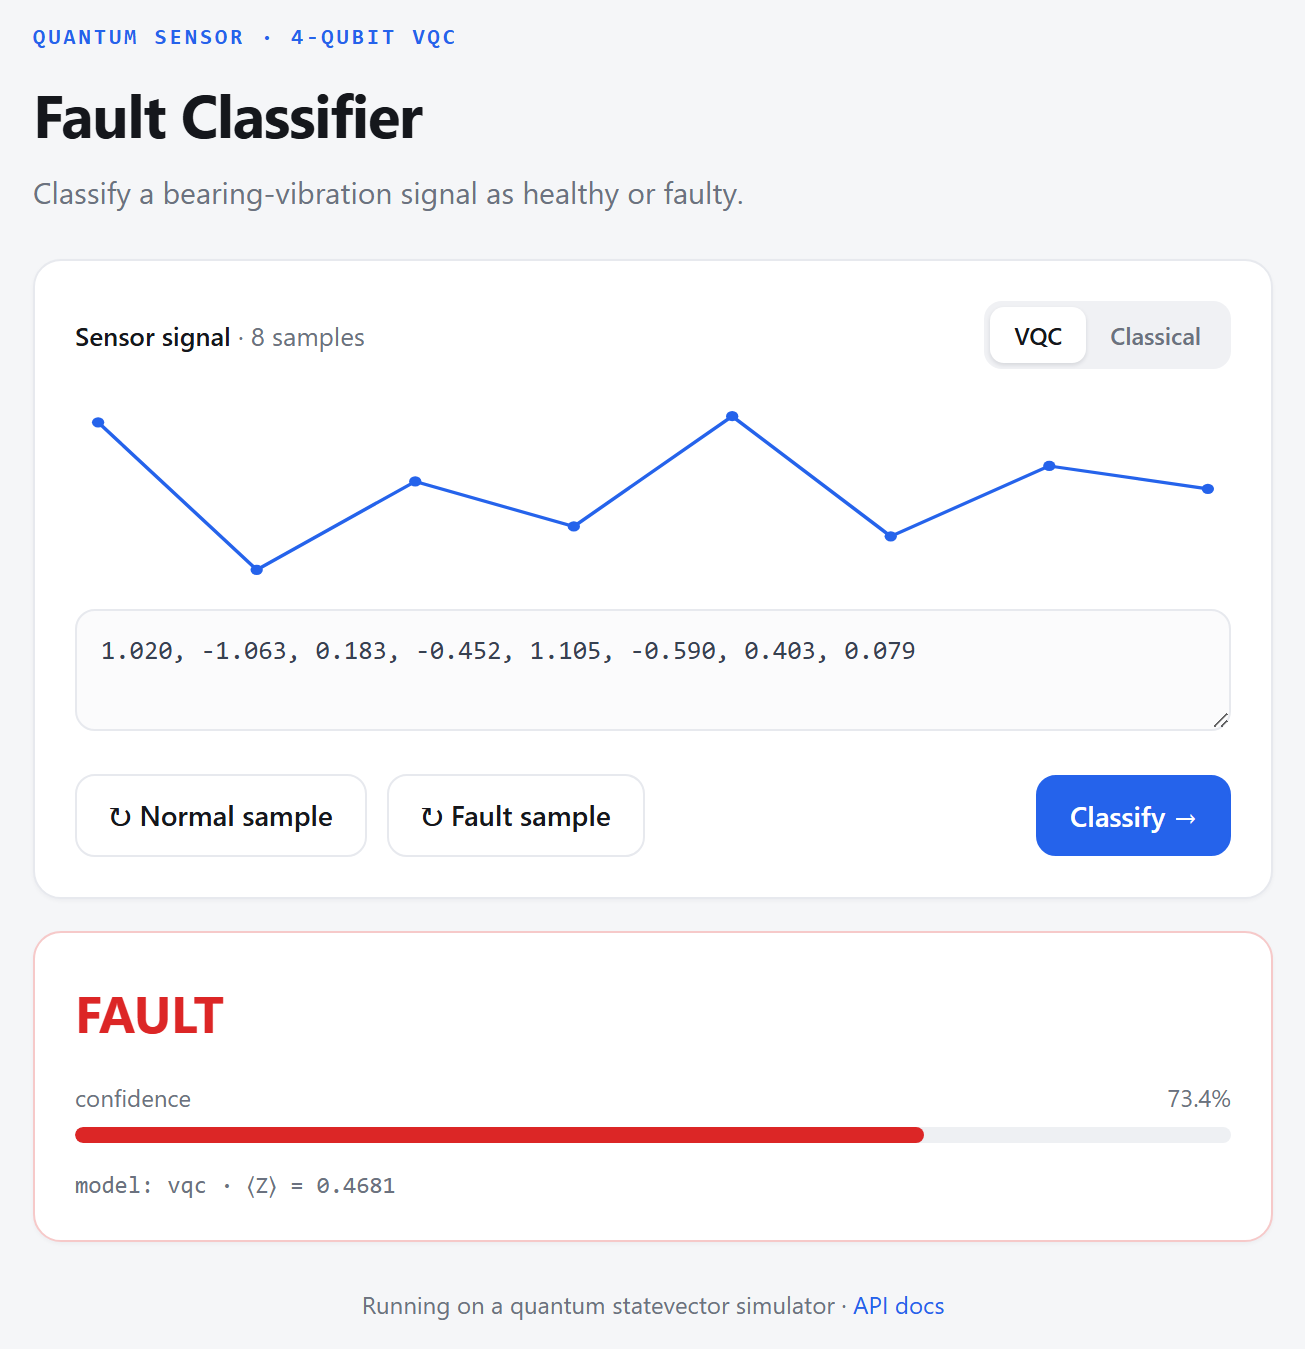
\includegraphics[width=0.82\columnwidth]{ui_app.png}
  \caption{The web app classifying a faulty signal: the input waveform, the
  verdict, a confidence bar, and the quantum $\langle Z\rangle$ output.}
  \label{fig:ui}
\end{figure}

\subsection{Install and run}
With Python~3.11, install the serving dependencies and start the service:
\begin{enumerate}
\item \texttt{pip install -r requirements-serve.txt}
\item \texttt{python -m qsensor.training} \,(trains once; saves to \texttt{artifacts/})
\item \texttt{uvicorn qsensor.api:app} \,(serves \texttt{http://localhost:8000})
\end{enumerate}
A containerised alternative is \texttt{docker compose up -{}-build}, and the full
endpoint reference is in \texttt{DEPLOY.md}.

% =====================================================================
\section{Challenges and Next Steps}\label{sec:disc}
A few changes did most of the work, and they are worth writing down.

\emph{Barren plateaus.} An early eight-qubit, fully entangled design trained to
only about 52\%, no better than guessing, because its gradients had vanished.
Dropping to four qubits with linear entanglement, a shallow ansatz, and a small
random start brought training back to life.

\emph{Encoding range.} Scaling features to $[0,\pi]$ let the ZZ angle products
reach $\pi^2\approx 9.9$\,rad, past $2\pi$, so the angles wrapped and the class
information was scrambled. Rescaling to $[0,1]$ removed the wrap and was the
first big jump in VQC accuracy, from below 60\% to the high 70s.

\emph{Readout and re-uploading.} The last gain came from the model itself:
replacing the parity-bit readout with a smooth average-$\langle Z\rangle$
expectation and re-uploading the data across three blocks. Trained with COBYLA on
the exact simulator, this lifted the VQC to 90.3\%, close to the quantum kernel.

For the next two months we plan to: repeat every run over several seeds with
cross-validation and report error bars; train directly under noise and compare
with the train-clean, test-noisy setup used here; add readout-error mitigation
and other ZNE fits; and, if the hardware queue allows, check the best setup on a
real IBM Quantum backend.

% =====================================================================
\section{Conclusion}
In one month we built a working, reproducible quantum pipeline for sensor fault
detection: a 97.2\% quantum-kernel classifier, a 90.3\% trained VQC, a clear
noise-resilience curve, and a ZNE mitigation step. The changes that mattered,
qubit count, encoding range, and a smooth expectation readout with data
re-uploading, are the kind of detail that separates a working quantum model from
a random one. The code and results are on GitHub and form the base for the
noise-aware study planned next.

% =====================================================================
\begin{thebibliography}{9}
\small
\bibitem{havlicek} V.~Havl\'i\v{c}ek \textit{et al.}, ``Supervised learning with
  quantum-enhanced feature spaces,'' \textit{Nature} \textbf{567}, 209--212 (2019).
\bibitem{mcclean} J.~R.~McClean \textit{et al.}, ``Barren plateaus in quantum
  neural network training landscapes,'' \textit{Nat.\ Commun.} \textbf{9}, 4812 (2018).
\bibitem{mitarai} K.~Mitarai \textit{et al.}, ``Quantum circuit learning,''
  \textit{Phys.\ Rev.\ A} \textbf{98}, 032309 (2018).
\bibitem{temme} K.~Temme, S.~Bravyi, and J.~M.~Gambetta, ``Error mitigation for
  short-depth quantum circuits,'' \textit{Phys.\ Rev.\ Lett.} \textbf{119}, 180509 (2017).
\bibitem{cerezo} M.~Cerezo \textit{et al.}, ``Variational quantum algorithms,''
  \textit{Nat.\ Rev.\ Phys.} \textbf{3}, 625--644 (2021).
\bibitem{qiskit} Qiskit Contributors, ``Qiskit: An Open-source Framework for
  Quantum Computing,'' 2024.
\end{thebibliography}

\end{document}
